\renewcommand*{\arraystretch}{1.1}

\noindent\begin{tabularx}{17cm}{|>{\small \sf}c|X|}
	\hline
	query    & BI / 1 \\ \hline
%
	title       & Posting summary \\ \hline
%
    pattern     & \hfill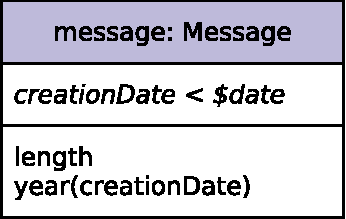
\includegraphics[scale=\patternscale,margin=0cm .2cm]{patterns/bi-read-01}\hfill\vadjust{} \\ \hline
%
	desc. & Given a date, find all Messages created before that date. Group them by
a 3-level grouping:

\begin{enumerate}
\def\labelenumi{\arabic{enumi}.}
\tightlist
\item
  by year of creation
\item
  for each year, group into message types, i.e., Posts or Comments
\item
  for each year-type group, split into four groups based on length of
  their content

  \begin{itemize}
  \tightlist
  \item
    0 \textless{}= length \textless{} 40: \texttt{short}
  \item
    40 \textless{}= length \textless{} 80: \texttt{one\ liner}
  \item
    80 \textless{}= length \textless{} 160: \texttt{tweet}
  \item
    160 \textless{}= length: \texttt{long}
  \end{itemize}
\end{enumerate}
 \\ \hline
%
	
	group by       &
	\multicolumn{1}{>{\raggedright}X|}{
		\varname{year}, 
		\varname{message type}, 
		\varname{length group}
		} \\ \hline
	
%
	params.  &
	\vspace{1.1ex}{\begin{tabularx}{14.2cm}{|c|M|m{2cm}|Y|} \hline
	\cellcolor{parameter} \color{white} $\mathsf{1}$ & \varname{date} & \cellcolor{gray!20} \vartype{Date} &  \\ \hline
	\end{tabularx}}\vspace{1.1ex} \\ \hline
%
	
	result      &
	\vspace{1.1ex}{\begin{tabularx}{14.2cm}{|c|M|m{2cm}|c|Y|} \hline
	\cellcolor{result} \color{white} $\mathsf{1}$ & \varname{messageYear} & \cellcolor{gray!20} \vartype{32-bit Integer} &
	    \texttt{R} &
	    year of the message \\ \hline
	\cellcolor{result} \color{white} $\mathsf{2}$ & \varname{messageType} & \cellcolor{gray!20} \vartype{String} &
	    \texttt{R} &
	    post/comment (in lowercase) \\ \hline
	\cellcolor{result} \color{white} $\mathsf{3}$ & \varname{lengthCategory} & \cellcolor{gray!20} \vartype{String} &
	    \texttt{C} &
	    short/one-liner/tweet/long (in lowercase) \\ \hline
	\cellcolor{result} \color{white} $\mathsf{4}$ & \varname{messageCount} & \cellcolor{gray!20} \vartype{32-bit Integer} &
	    \texttt{A} &
	    total number of Messages (Posts/Comments) in that group \\ \hline
	\cellcolor{result} \color{white} $\mathsf{5}$ & \varname{averageMessageLength} & \cellcolor{gray!20} \vartype{32-bit Integer} &
	    \texttt{A} &
	    average length of the Message content in that group \\ \hline
	\cellcolor{result} \color{white} $\mathsf{6}$ & \varname{sumMessageLength} & \cellcolor{gray!20} \vartype{32-bit Integer} &
	    \texttt{A} &
	    sum of all message content lengths \\ \hline
	\cellcolor{result} \color{white} $\mathsf{7}$ & \varname{percentageOfMessages} & \cellcolor{gray!20} \vartype{32-bit Float} &
	    \texttt{A} &
	    number of messages in group as a percentage of all messages created before the given date \\ \hline
	\end{tabularx}}\vspace{1.1ex} \\ \hline
	
%
	sort        &
	\vspace{1.1ex}{\begin{tabular}{|c|l|c|} \hline
	\cellcolor{sort} \color{white} $\mathsf{1}$ & \varname{year} & \cellcolor{gray!20} $\desc$ \\ \hline
	\cellcolor{sort} \color{white} $\mathsf{2}$ & \varname{message type} & \cellcolor{gray!20} $\asc$ \\ \hline
	\cellcolor{sort} \color{white} $\mathsf{3}$ & \varname{size category} & \cellcolor{gray!20} $\asc$ \\ \hline
	\end{tabular}}\vspace{1.1ex} \\ \hline
	%
	%
	CPs &
	\multicolumn{1}{>{\raggedright}l|}{
	  \chokepoint{1.2}, 
	  \chokepoint{3.2}, 
	  \chokepoint{4.1}
	  } \\ \hline
	%
    %
\end{tabularx}
\vspace{2ex}